\documentclass[11pt,spanish]{article}

\usepackage{listings}             
\usepackage{anysize} 
\usepackage{graphicx}
\usepackage[spanish]{babel}
\usepackage[utf8]{inputenc}
\usepackage{xcolor}
\usepackage{wrapfig}

\lstset{language=Python}
\marginsize{1cm}{1cm}{2cm}{2cm}
\selectlanguage{spanish}
\lstset{
language=Python,
 backgroundcolor=\color{red!75!green!50!blue!25},
 frame=single,
literate=
  {á}{{\'a}}1 {é}{{\'e}}1 {í}{{\'i}}1 {ó}{{\'o}}1 {ú}{{\'u}}1
  {Á}{{\'A}}1 {É}{{\'E}}1 {Í}{{\'I}}1 {Ó}{{\'O}}1 {Ú}{{\'U}}1
  {à}{{\`a}}1 {è}{{\`e}}1 {ì}{{\`i}}1 {ò}{{\`o}}1 {ù}{{\`u}}1
  {À}{{\`A}}1 {È}{{\'E}}1 {Ì}{{\`I}}1 {Ò}{{\`O}}1 {Ù}{{\`U}}1
  {ä}{{\"a}}1 {ë}{{\"e}}1 {ï}{{\"i}}1 {ö}{{\"o}}1 {ü}{{\"u}}1
  {Ä}{{\"A}}1 {Ë}{{\"E}}1 {Ï}{{\"I}}1 {Ö}{{\"O}}1 {Ü}{{\"U}}1
  {â}{{\^a}}1 {ê}{{\^e}}1 {î}{{\^i}}1 {ô}{{\^o}}1 {û}{{\^u}}1
  {Â}{{\^A}}1 {Ê}{{\^E}}1 {Î}{{\^I}}1 {Ô}{{\^O}}1 {Û}{{\^U}}1
  {œ}{{\oe}}1 {Œ}{{\OE}}1 {æ}{{\ae}}1 {Æ}{{\AE}}1 {ß}{{\ss}}1
  {ű}{{\H{u}}}1 {Ű}{{\H{U}}}1 {ő}{{\H{o}}}1 {Ő}{{\H{O}}}1
  {ç}{{\c c}}1 {Ç}{{\c C}}1 {ø}{{\o}}1 {å}{{\r a}}1 {Å}{{\r A}}1
  {€}{{\EUR}}1 {£}{{\pounds}}1
}


\title{\vspace{-3cm}\begin{flushleft}\textbf{Actividad 6}\end{flushleft}}
\author{\hspace{-9.6cm}\textsc{Andrés Ignacio Rodríguez Mendoza}}
\date{}

\begin{document}

\begin{wrapfigure}{r}{0.2\textwidth}
  \begin{center}
   \vspace{-5.4cm} 
\includegraphics[width=0.15\textwidth]{uni}
  \end{center}
\end{wrapfigure}

\maketitle  
\begin{center}
\rule{\textwidth}{1pt}
\end{center}


\section*{Introducción}

La ecuación diferencial se facilita considerando ángulos más pequeños que un radián, es decir, $\theta \ll  1$, por lo cual, $\sin \theta \approx \theta$. Reemplazando esto en la ecuación diferencial, queda,
$$\frac{d^2\theta}{dt^2} + \frac{g}{l} \theta = 0.$$
Dadas las condiciones iniciales $\theta (0) = \theta _ 0$ y $d\theta / dt (0) =0$, la solución es,
$$\theta (t) = \theta _0 \cos \left( \sqrt{\frac{g}{l} t} \right)$$
El movimiento es armónico simple, donde $\theta_0$ es la semiamplitud de oscilación. El periodo del movimiento es,
$$T_0 = 2 \pi \sqrt{\frac{l}{g}}.$$
Para amplitudes más grandes que la aproximación a ángulos pequeños, se puede calcular el periodo invirtiendo la ecuación de la velocidad angular,
$$\frac{dt}{d\theta}=\frac{l}{2g} \frac{1}{\sqrt{\cos \theta - \cos \theta_0}}$$
e integrando sobre un ciclo completo,
$$ T= t(\theta _0 \rightarrow 0 \rightarrow -\theta_0 \rightarrow 0 \rightarrow \theta_0),$$
o dos veces un medio ciclo,
$$ T= 2t(\theta _0 \rightarrow 0 \rightarrow -\theta_0),$$
o cuatro veces un cuarto de ciclo,
$$ T= 2t(\theta _0 \rightarrow 0),$$
que nos lleva a
$$T= 4 \sqrt{\frac{l}{2g}} \int ^{\theta _0} _0 \frac{1}{\sqrt{\cos\theta - \cos\theta_0}} d\theta.$$
Nótese que esta integral diverge como $\theta_0$ se aproxime a la vertical. Así, con la energía adecuada, un péndulo en su máximo podría tomar un tiempo arbitrariamente largo para caer.\\ \\
Para resolver numericamente esta integral se utiliza \textit{Scipy.integrate.quad} para integrales definidas de la biblioteca de funciones \textit{Scipy.integrate} en Python. Para mostrar que la integral diverge cuando el ángulo inicial tiene a $\pi$ se resuelve la integral desde cero hasta $\pi$. Los resultados se comparan con el periodo de la aproximación a ángulos pequeños.

\section*{Código}



\begin{lstlisting}

import numpy as np
from scipy import integrate
import matplotlib.pyplot as plt


n=1000

# Arreglos 
x=[]
TT0=[]
x_0=np.linspace(0.001,np.pi + 0.001, n)



#   el integrando
I = lambda x,a: 1/np.sqrt(np.cos(x) - np.cos(a))


for i in range(n):
#   la integral
    theta_0=x_0[i]
    T , err= integrate.quad(I, 0, theta_0, args=(theta_0,))
    
    
#   el error
    TT0.append(np.sqrt(2)/np.pi * T)
    
    
    
#   Gráfica desviación
plt.figure(1)
plt.plot(x_0 * 180 / np.pi, TT0 , "r" )
plt.title('Desviación periodo real - aproximación')
plt.xlabel(r'$ \theta _0 (deg)$')
plt.ylabel("T/To")
plt.xlim(0,90)
plt.ylim(1,1.2)
plt.grid()


plt.show()


#   Gráfica divergencia
plt.figure(1)
plt.plot(x_0 * 180 / np.pi, TT0 , "b" )
plt.title('Divergencia en ' r'$\theta_0 = \pi$')
plt.xlabel(r'$ \theta _0 (deg)$')
plt.ylabel("T/To")
plt.xlim(0,180)
plt.ylim(1,5)
plt.grid()


plt.show()

\end{lstlisting}

\section*{Gráficas}

\centering

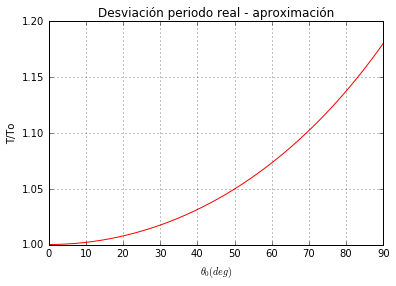
\includegraphics{plot}\\
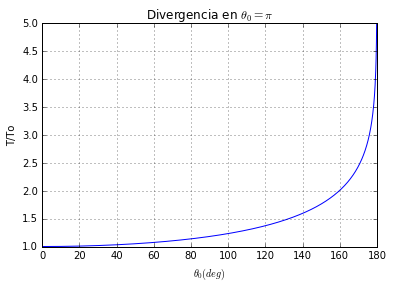
\includegraphics{plot2}\\







\end{document}


